\documentclass[a4paper,12pt]{article}


% add more packages if necessary
\usepackage{xspace}
\usepackage{graphicx}
\usepackage{xcolor}
\usepackage{hyperref}
\usepackage{epstopdf}

% TODO: Add your group name
\newcommand{\groupname}{Badgers\xspace}


\title{
Project Report \\ 
Group \groupname \\
\vspace{5mm}
\large Java and C\# in depth, Spring 2013
}
\author{
% TODO: Add your names here
Thomas Frick (03-150-927)\\
Matthias Ganz (04-862-850)\\
Philipp Rohr (04-397-030)
}
\date{\today}



\begin{document}
\maketitle


\section{Introduction}

This document describes the design and implementation of the \emph{Personal
Virtual File System} of group \emph{\groupname}. The project is part of the
course \emph{Java and C\# in depth} at ETH Zurich. The following sections
describe each project phase, listing the requirements that were implemented and
the design decisions taken. The last section describes a use case of using the
\emph{Personal Virtual File System}.

% PART I: VFS CORE
% --------------------------------------

\section{VFS Core}

% TODO: Remove this line
%\textbf{[This section has to be completed by April 8th.]}

%TODO: Remove this text and replace it with actual content

VFS Core is a library that provides an implementation of a virtual file system.
The API that a client of this library can use consists of three interfaces that
are described in \ref{sec:coreClasses}. The VFS Core provides functionality to
create/open/dispose new virtual disks and allows the management of files and
directories within such a disk. Furthermore it provides a simple way to
import/export files from/to the host file system.

The library internally works with a virtual disk that is divided into a header,
index and data section, having the index represented as B-tree. Such a design
allows with good performance access to the data on the disk.

\subsection{Requirements}
Below one will find a list of the requirements implemented in this project.

\subsubsection {disk management}
\begin{itemize}
  \item \emph{The virtual disk must be stored in a single file in the working
  directory in the host file system.}
  \item \emph{VFS must support the creation of a new disk with the specified
  maximum size at the specified location in the host file system. }
  \item \emph{VFS must support several virtual disks in the host file system.}
  \item \emph{VFS must support disposing of the virtual disk.}
  \item \emph{VFS must support querying of free/occupied space in the virtual
  disk.}
\end{itemize}  These requirements are met with the classes
\begin{verbatim}
ch.eth.jcd.badgers.vfs.core.VFSDiskManagerImpl
ch.eth.jcd.badgers.vfs.core.config.DiskConfiguration
\end{verbatim} allow creation/deletion and opening of the disk on the host
file system. Clients of the library have to pass a \textit{DiskConfiguration}
to the \textit{VFSDiskManagerImpl} when calling \textit{create} or
\textit{open}
\subsubsection{file management}
\begin{itemize}
  \item \emph{VFS must support creating/deleting/renaming directories and files.}
  \item \emph{VFS must support navigation: listing of files and folders, and
  going to a location expressed by a concrete path.}
  \item \emph{VFS must support moving/copying directories and files, including
  hierarchy.}
  \item \emph{VFS must support importing files and directories from
  the host file system.}
  \item \emph{VFS must support exporting files and directories to the host file
  system.}
\end{itemize} These requirements are met with the classes
\begin{verbatim}
ch.eth.jcd.badgers.vfs.core.VFSEntryImpl
ch.eth.jcd.badgers.vfs.core.VFSPathImpl
ch.eth.jcd.badgers.vfs.core.VFSFileInputStream
ch.eth.jcd.badgers.vfs.core.VFSFileOutputStream
\end{verbatim}The \textit{VFSEntryImpl} allows
copy, move (and rename), delete, listing of children and going to the parent
(navigation). Together with the streams it also supports importing/exporting
to any location clients of the VFS core library wish to. The classes
\begin{verbatim}
ch.eth.jcd.badgers.vfs.ui.VFSConsole
ch.eth.jcd.badgers.vfs.ui.VFSUIController
\end{verbatim} demonstrate this by importing and exporting to the host file
system.

\subsubsection {bonus features}
\begin{itemize}
  \item \emph{Elastic disk: Virtual disk can dynamically grow or shrink,
  depending on its occupied space.}
\end{itemize}
The implementation only allows growing if more files are imported. Shrinking is
not supported.

\begin{itemize}
  \item \emph{Compression, if implemented with 3d party library.}
  \item \emph{Compression, if implemented by hand (you can take a look at
  the arithmetic compression)}
\end{itemize}

The classes
\begin{verbatim}
ch.eth.jcd.badgers.vfs.compression.BadgersLZ77CompressionInputStream
ch.eth.jcd.badgers.vfs.compression.BadgersLZ77CompressionOutputStream
ch.eth.jcd.badgers.vfs.compression.BadgersRLECompressionInputStream
ch.eth.jcd.badgers.vfs.compression.BadgersRLECompressionOutputStream
\end{verbatim}
implement streams that can be wrapped around \textit{VFSFileInputStream} and
\textit{VFSFileOutputStream}. The \textit{DiskConfiguration} allows
to switch compression on and to declare which algorithm shall be chosen. This
allows easy configuration of any 3rd party compression streams (which was not
chosen to implement, because of the implementation of our own compression
algorithm).

\begin{itemize}
  \item \emph{Encryption, if implemented with 3rd party library.}
  \item \emph{Encryption, if implemented by hand.}
\end{itemize}

The classes
\begin{verbatim}
ch.eth.jcd.badgers.vfs.encryption.CaesarInputStream
ch.eth.jcd.badgers.vfs.encryption.CaesarOutputStream
\end{verbatim}
show how encryption can be implemented in the library. It was chosen to
implement encryption similar to compression with streams, which allows easy
configuration via \textit{DiskConfiguration}. These streams are mainly for
demonstration how encryption should work and shall not be used in high
security environments :-)

\subsection{Design}
This section describes the main aspects of the VFS core library. It shows the
implementation of the core interfaces and classes, explains the mock classes and
tests and eventually describes the file format and its management classes.

\subsubsection{Core Classes}\label{sec:coreClasses}
Figure \ref{fig:core_classes} gives an overview of the main interfaces and
classes that were implemented. The interfaces \textit{VFSDiskManager},
\textit{VFSEntry} and \textit{VFSPath} can be used by clients using the library
implemented here.
\begin{itemize}
\item{\textit{VFSDiskManager}} The implementations of this interface provide
mainly a way to open, create and dispose new virtual disks. Additionally one can
get the root entry of the file system and get additional information about an
opened disk.
\item{\textit{VFSEntry}} Represents a directory or file on the file system. A
\textit{VFSEntry} provides all the required methods to manipulate files and
directories and importing/exporting files into the virtual file system. The
general meaning of \textit{VFSEntry} is, that such objects usually exist on the
filesystem.
\item {\textit{VFSPath}} Represents a path on the file system to a given
\textit{VFSEntry}. It has a slightly looser coupling to the file system as a
path does not imperatively need to exist.
\end{itemize}

The intention of those interfaces is to hide the real implementation of the
virtual file system from a client. With that in mind it should be simple to add
a network layer upon the real implementation without changing client code. The
classes \textit{VFSDiskManagerImpl, VFSEntryImpl (and its descendants) and
VFSPathImpl} implement all the management for actually using the VFS on a virtual disk.

\begin{figure}[h!]
\centering
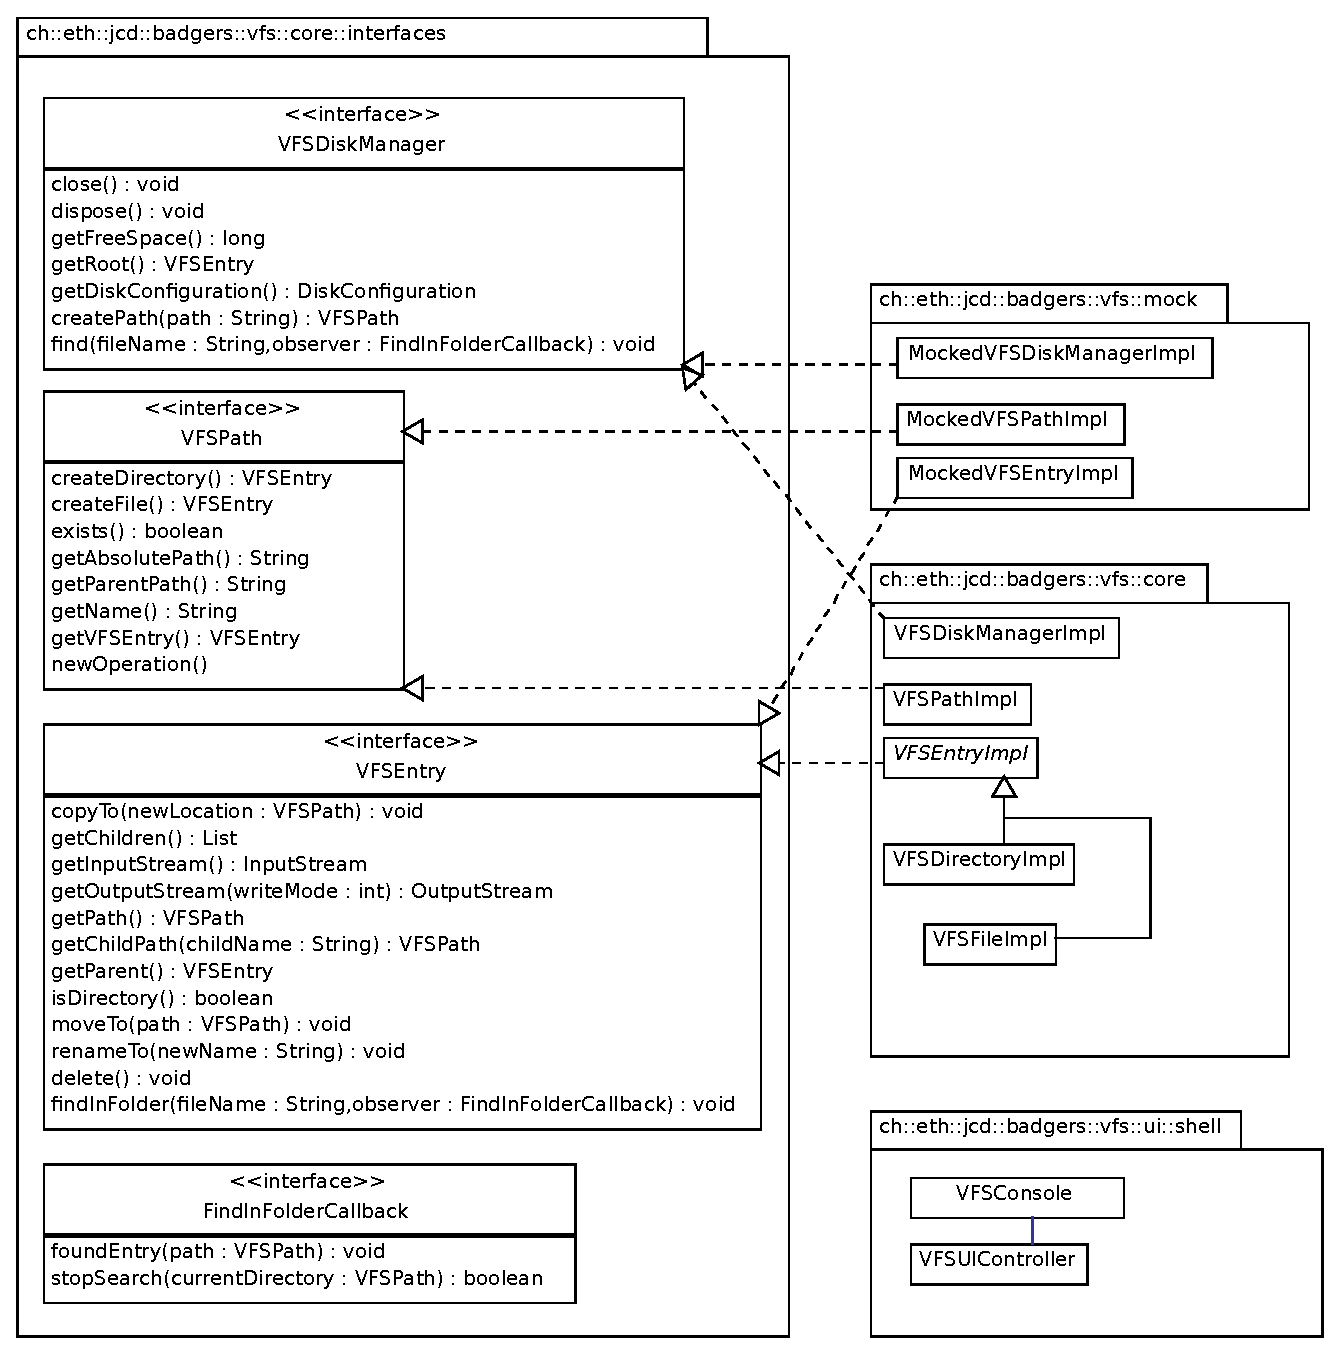
\includegraphics[width=1\textwidth]{figures/core_classes.eps}
\caption{core classes}
\label{fig:core_classes}
\end{figure}

\subsubsection{Mocking}
For discussing the semantics of the virtual file system and the development of 
the interfaces explained in \ref{sec:coreClasses} it was decided to implement a mock
that works against the host file system. The mock classes implement all
the interfaces and were very helpful for acquiring a common understanding of how
the interface shall be used by clients. In a further step it was very useful to have
the mock classes while developing the console application which could be
developed independently from the real implementation.
\subsubsection{Test}
During the development a bunch of test cases came to life. The tests solely
depend on the interfaces and thus they can run against the mock classes and the
real implementation. This was a huge help in finding bugs in the slightly more
complicated real implementation.
\subsection{The \emph{real} implemenation}

Eventually some code that handles a virtual disk was developed and is described
in this section.

\subsubsection{The File Format}


This section describes the binary file format used by the file system inside a
virtual disk.
The file is separated into three major parts. The header, index and the data
section. Each of them is described below.

\begin{figure}[h!]
\centering
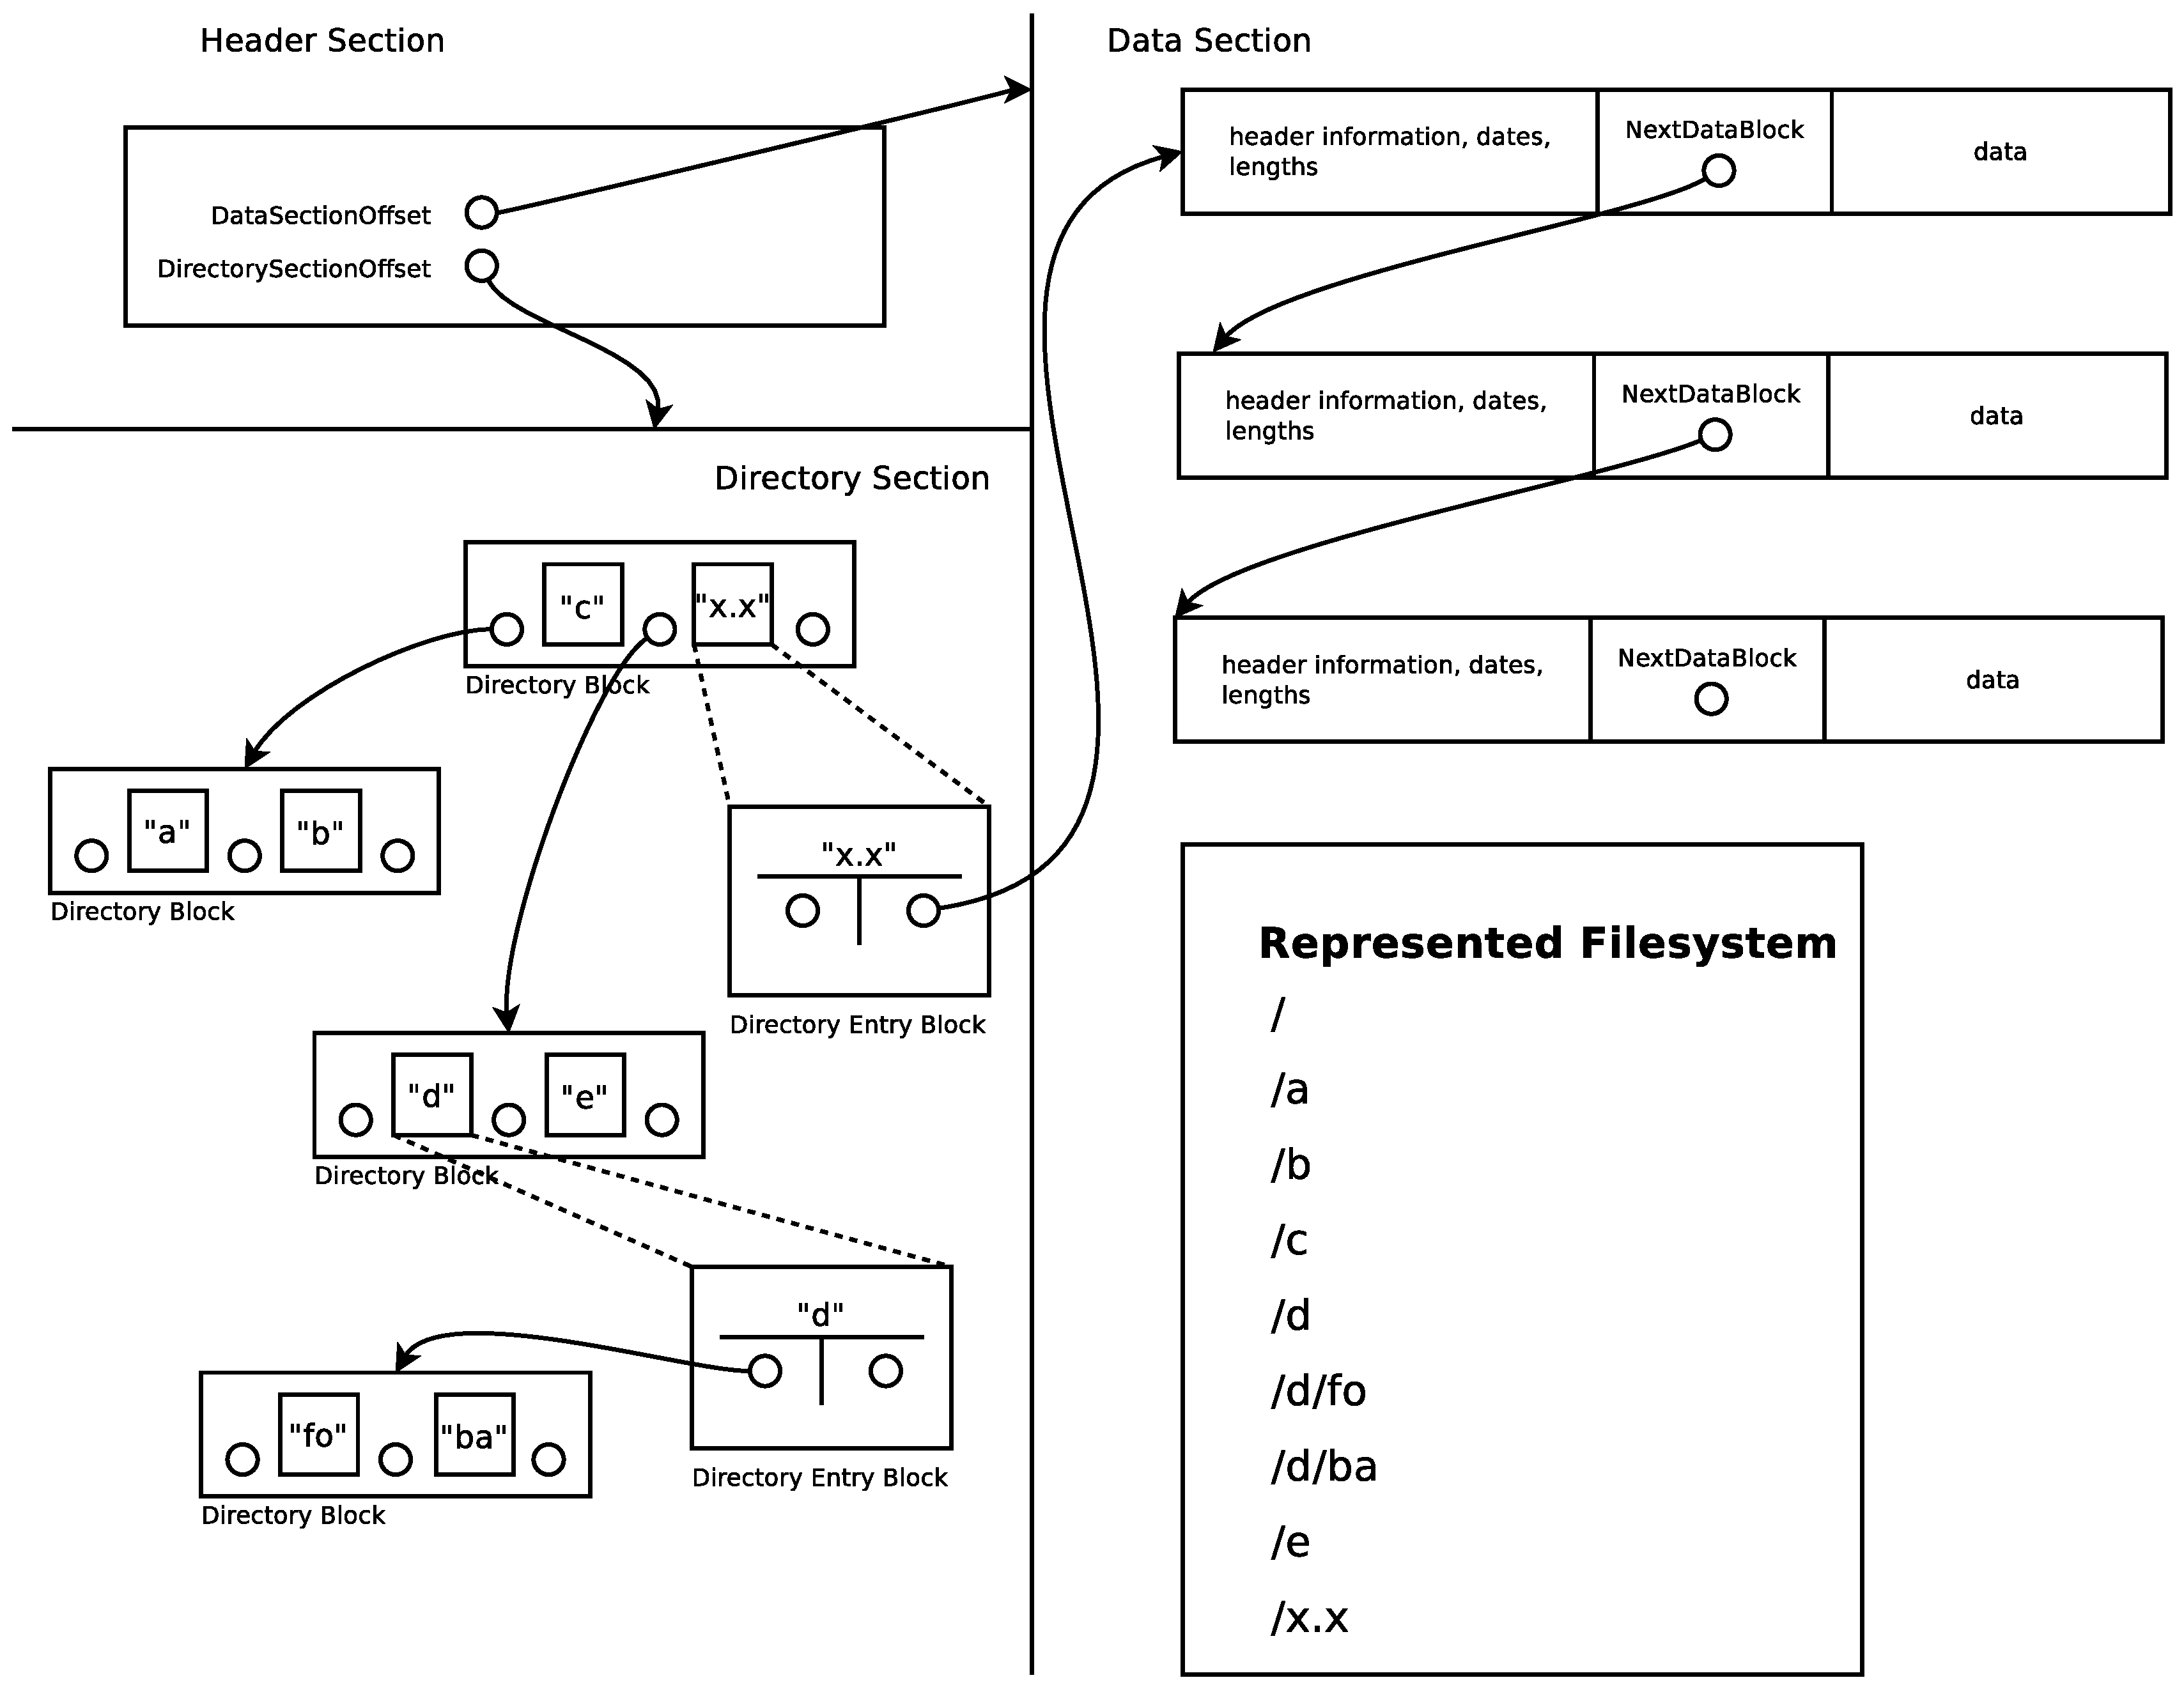
\includegraphics[width=1\textwidth]{figures/fileFormat.eps}
\caption{Overview of a disk}
\label{fig:disk_overview}
\end{figure}

\paragraph{Header Section} The header section contains some general information
about the currently opened virtual disk. The details can be found in the
following table:

\begin{tabular}{|l|l|p{5cm}|}
\hline
  \textbf{Name} & \textbf{Length} & \textbf{Description}
\\  \hline
  Info & 50 byte UTF-8 String & Contains something like Badger VFS 2013 V1.0 
\\ \hline
  Version & 10 byte UTF-8 String & Contains something like "1.0"
\\ \hline
  Compression used & 20 byte UTF-8 String & null or indicates compression used for this file
\\ \hline
  Encryption used & 20 byte UTF-8 String & null or indicates encryption used for this file
\\ \hline
 DirectorySectionOffset & long (8 byte) &  File offset where our directory section
 starts \\ \hline
 DataSectionOffset & long (8 byte) &  File offset where our data section starts
\\ \hline
 SaltString & 8 bytes  & Salt used to hash username and password randomly string generated while creating this
   file
 \\ \hline
  Password & xxx bytes  & CryptoHash (SHA-whatever) of Password+SaltString
\\ \hline

\end{tabular}


\paragraph{Directory Section}

The directory section describes which files and folders belong to which parent directory. This section has a fixed size and contains so called DirectoryBlocks which also have a fixed size. This makes management an manipulation easy. To each directory belongs a B-Tree structure which lists all contained entries.


\subparagraph*{Directory Block}

One Directory Block represents a Node in our B-Tree of order 2.

\begin{tabular}{|l|l|p{5cm}|}
\hline
  \textbf{Name} & \textbf{Length} & \textbf{Description}
\\  \hline

DirectoryHeader & 1 byte & Header information. This header makes it easy to determine whether a DirecotryBlock is in used or not (memory management)

\\  \hline

DirectoryEntryBlock1 & 128 byte & The smaller key inserted into our B-Tree

\\  \hline

DirectoryEntryBlock2 & 128 byte & The bigger key inserted into our B-Tree

\\  \hline

DirectoryBlockLink1 & 8 byte & Points to another DirectoryBlock which contains keys smaller than DirectoryEntryBlock1

\\  \hline

DirectoryBlockLink2 & 8 byte & Points to another DirectoryBlock which contains keys bigger than DirectoryEntryBlock1 but smaller than DirectoryEntryBlock2

\\  \hline

DirectoryBlockLink3 & 8 byte & Points to another DirectoryBlock which contains keys bigger than DirectoryEntryBlock2

\\  \hline


\end{tabular}

\subparagraph*{Directory Entry Block}

Represents a single directory or file.

\begin{tabular}{|l|l|p{5cm}|}
\hline
  \textbf{Name} & \textbf{Length} & \textbf{Description}
\\  \hline

Filename & 112 byte & UTF-8 Filename String 


\\  \hline

DataBlockLocation & 8 byte & Pointer to a DataBlock located in the Data Section.
This DataBlock holds some meta information about the current directory


\\  \hline

DirectoryEntryTreeRoot & 8 bytes & Pointer to a DirectoryBlock located in the
Directory Section. This referenced DirectoryBlock is the Root Block of a B-Tree
containing all entries of that directory specified by the current Directory Entry Block.
\newline

\textbf{This field containing a 0 indicates that this entry is a file not a directory}



\\  \hline

\end{tabular}


\paragraph{Data Section}
The data section is split into blocks where each of them is X bytes long.
Each block contains some amount of data and points to a subsequent block


Block layout \\

\begin{tabular}{|l|l|p{5cm}|}
\hline
  \textbf{Name} & \textbf{Length} & \textbf{Description}
\\  \hline
 BlockHeader & 1 byte & 
 \\
 \hspace{0.2cm} 0) Header-Bit (LSB) & &  If set to 1 this is the first datablock
 of a file.
 \\ 
 \hspace{0.2cm} 1) not used & &  
 \\ 
 \hspace{0.2cm} 2) not used & &  
 \\ 
 \hspace{0.2cm} 3) not used & &  
 \\ 
 \hspace{0.2cm} 4) not used & &  
 \\ 
 \hspace{0.2cm} 5) not used & &  
 \\ 
 \hspace{0.2cm} 6) not used & &  
 \\ 
 \hspace{0.2cm} 7) not used & &  
 
\\  \hline
 NextDataBlock & 8 byte & 
 Points to the start address of the next Datablock (linked list).
    0 if this is the last DataBlock of a certain file or folder.
\\  \hline
  CreationDate & 8 byte & UTC Time when this file was created
  \newline \textit{This field only exists if Header-Bit is set to 1}
\\  \hline

  DataLength & 4 byte &
    Indicates the number of data saved on this DataBlock.
    
\\  \hline
 Data & n byte & user data (may be encrypted/compressed)
\\  \hline
\end{tabular}


\paragraph{The root directory}


\subsubsection{compression layer}

To reduce the data volume within the virtual disk, compression on each file can
be enabled. Currently available compression algorithms are run length encoding
\cite{rle} and LZ77 \cite{lz77}.

\paragraph{Run Length Encoding}

The available 8bit run length encoding(rle) algorithm is a very simple form of
data compression where multiple occurrence of the same byte were stored as a
single byte value and the corresponding count. It is useful for simple graphic
images like line drawings and icons.

\paragraph{LZ77}

Abraham Lempel and Jacob Ziv introduced the LZ77 lossless compression algorithm
in 1977. Newer compression methods such as GZIP or DEFLATE often use LZ77-based
algorithms. The compression is achieved by replacing the data with a reference
to an earlier existing copy in the data input stream. For that a window of
a certain size is held in memory where existing copies of the current data are
searched.


% PART II: VFS Browser
% --------------------------------------

%\section{VFS Browser}

% TODO: Remove this line
%\textbf{[This section has to be completed by April 22nd.]}

%TODO: Remove this text and replace it with actual content
%\emph{Give a short (1-2 paragraphs) description of what VFS Browser is.}


%\subsection{Requirements}

% TODO: Remove this text and replace it with actual content
%\emph{Describe which requirements (and possibly bonus requirements) you have
% implemented in this part. Give a quick description (1-2 sentences) of each requirement. List the software elements (classes and or functions) that are mainly involved in implementing each requirement.}


%\subsection{Design}

% TODO: Remove this text and replace it with actual content
%\emph{Give an overview of the design of this part and describe in general terms
% how the implementation works. You can mention design patterns used, class diagrams, definition of custom file formats, network protocols, or anything else that helps understand the implementation.}


%\subsection{Integration}

% TODO: Remove this text and replace it with actual content
%emph{If you had to change the design or API of the previous part, describe the
%changes and the reasons for each change here.}



% PART III: Synchronization Server
% --------------------------------------

%\section{Synchronization Server}

% TODO: Remove this line
%\textbf{[This section has to be completed by May 13th.]}

%TODO: Remove this text and replace it with actual content
%\emph{Give a short (1-2 paragraphs) description of what VFS Browser is.}


%\subsection{Requirements}

% TODO: Remove this text and replace it with actual content
%\emph{Describe which requirements (and possibly bonus requirements) you have
% implemented in this part. Give a quick description (1-2 sentences) of each requirement. List the software elements (classes and or functions) that are mainly involved in implementing each requirement.}


%\subsection{Design}

% TODO: Remove this text and replace it with actual content
%\emph{Give an overview of the design of this part and describe in general terms
% how the implementation works. You can mention design patterns used, class diagrams, definition of custom file formats, network protocols, or anything else that helps understand the implementation.}


%\subsection{Integration}

% TODO: Remove this text and replace it with actual content
%\emph{If you had to change the design or API of the previous part, describe the
% changes and the reasons for each change here.}





% TODO: Remove this line
%\textbf{[optional: This part has to be completed by April 8th.]}

% TODO: Remove this text and replace it with actual content

% PART IV: Quick Start Guide
% --------------------------------------

\section{Quick Start Guide}


\subsection{the eclipse project}
The project requires to be compiled with JAVA 7. It also depends on the maven
plugin which pulls in all the required libraries.

\subsection{Command line client}

The command line client allows the usage of the VFS core and is mainly intended
to test the basic functionalities. The console runs either in  management mode
or in file system mode. The management mode is entered automatically when
starting the command line client. It allows creating and opening virtual
disks. The file system mode is entered as soon as a virtual disk is opened.

%\textbf{TODO: DISCUSSION: sollen ganze ordner importiert und exportiert werden
%können? wird dies von der client-seite gehandelt?}

\subsubsection{startup}
The command line client can be started as follows:

\begin{verbatim}
java -jar VFSCore.jar ch.eth.jcd.badgers.vfs.ui.shell.VFSConsole
\end{verbatim}

or by starting \verb|ch.eth.jcd.badgers.vfs.ui.shell.VFSConsole| in eclipse.



This gives a console prompt where the following commands can be used in.

\subsubsection{commands}
Following commands can be used with the command line client in management mode:

\begin{itemize}
  \item{\textbf{create c:\textbackslash path\textbackslash to\textbackslash
  disk.bfs [size]}} creates virtual disk with a maximum quota of [size]
  megabytes on the host system. The file may grow up to [size] megabytes. There
  is currently no way to change encryption or compression by using the console
  application. By default no encryption and the LZ77 compression will be used.
  \item {\textbf{open c:\textbackslash path\textbackslash to\textbackslash
  disk.bfs}} opens filesystem mode for the given virtual disk
  \item {\textbf{exit}} exits the console program
\end{itemize}

following commands can be used in file system mode:

\begin{itemize}
  \item {\textbf{ls}} lists the contents of the current directory
  \item {\textbf{pwd}} shows the path to the current directory
  \item {\textbf{df}} shows the usage of the current virtual disk space
  \item {\textbf{cd dst}} changes current directory to \textit{dst} which must
  be either a child directory of the current path or ``..''
  \item {\textbf{find searchString}} lists absolute paths of all files
  containing \textit{searchString} in their file name
  \item {\textbf{mkdir dirName}} creates a new directory \textit{dirName} in the
  current path
  \item {\textbf{mkfile fileName}} creates a new empty file \textit{fileName} in
  the current path - this is rather not useful, as the ``import'' creates a
  file with content
  \item {\textbf{rm file}} deletes the entry denoted as \textit{file}, it must
  be a child of the current path
  \item {\textbf{cp src dst}} copies the \textit{src} file to \textit{dst} as a
  child of the current path
  \item {\textbf{mv src dst}} moves the \textit{src} file to \textit{dst}
  \item {\textbf{import ext\_src dst}} imports a \textit{ext\_src} from the
  host system to \textit{dst}
  \item {\textbf{export src ext\_src}} exports a \textit{src} file to the host
  system \textit{ext\_dst}
  \item {\textbf{find searchString}} lists all filesystem entries below the
  current entry containing \textit{searchString}
  \item {\textbf{dispose}} deletes the currently opened virtual disk
  \item {\textbf{close}} closes the file system mode, from now on management mode
  commands can be executed
\end{itemize}
%\emph{If you have a command line interface for your VFS, describe here the
% commands available (e.g. ls, copy, import).} \\ \\ \\

\section{Glossary}

\paragraph{VFS core} The main Java library, that handles all the interaction
with virtual disks and importing/exporting/storing files. It is used by the
command line client and the GUI.

\paragraph{Virtual Disk} A virtual disk denotes a container file that is stored
on the host file system. A virtual disk can be opened with the software that is
developed during this project and stores the actual files. The file extension of
the virtual disk is ``*.bfs''.

% TODO: Remove this line
%\noindent\textbf{[This part has to be completed by May 13th.]}

% TODO: Remove this text and replace it with actual content
%\emph{Describe how to realize the following use case with your system. Describe
%the steps involved and how to perform each action (e.g. command line executions
% and arguments, menu entries, keyboard shortcuts, screenshots). The use case is the following:
%\begin{enumerate}
%\item Start synchronization server on localhost.
%\item Create account on synchronization server.
%\item Create two VFS disks (on the same machine) and link them to the new
% account.
%\item Import a directory (recursively) from the host file system into Disk 1.
%\item Dispose Disk 1 after the synchronization finished.
%\item Export the directory (recursively) from Disk 2 into the host file system.
%\item Stop synchronization server.
%\end{enumerate}
%}

\bibliographystyle{plain}
\bibliography{literature}
\end{document}
